%%%%%%%%%%%%%%%%%%%%%%%%%%%%%%%%%%%%%%%%%%%%%%%%%%%%%%%%%%%%%%%%%%%%%%%%%%%%%%%%%%
\begin{frame}[fragile]\frametitle{}
\begin{center}
{\Large Bokeh}

(Ref: Creating Interactive Visualizations with Bokeh - Fonnesbeck)
\end{center}
\end{frame}

%%%%%%%%%%%%%%%%%%%%%%%%%%%%%%%%%%%%%%%%%%%%%%%%%%%
\begin{frame}[fragile] \frametitle{What is Bokeh?}
\begin{itemize}
\item Bokeh is a Python package for creating interactive, browser-based visualizations
\item High-level commands for data binding, transformation, interaction
\item Low-level power to deeply customize
\end{itemize}
\end{frame}

%%%%%%%%%%%%%%%%%%%%%%%%%%%%%%%%%%%%%%%%%%%%%%%%%%%
\begin{frame}[fragile] \frametitle{How does Bokeh work?}
\begin{itemize}
\item Bokeh writes to a custom-built HTML5 Canvas library, which affords it high performance. 
\item This allows it to integrate with other web tools, such as Google Maps.
\item Bokeh plots are based on visual elements called glyphs that are bound to data objects.
\end{itemize}
\end{frame}

%%%%%%%%%%%%%%%%%%%%%%%%%%%%%%%%%%%%%%%%%%%%%%%%%%%
\begin{frame}[fragile] \frametitle{A Simple Example}
\begin{lstlisting}
import bokeh.plotting as bk

import numpy as np

x = np.linspace(-6, 6, 100)
y = np.random.normal(0.3*x, 1)
bk.circle(x, y, color="red", plot_width=500, plot_height=500)
bk.show()
\end{lstlisting}
\end{frame}

%%%%%%%%%%%%%%%%%%%%%%%%%%%%%%%%%%%%%%%%%%%%%%%%%%%
\begin{frame}[fragile] \frametitle{Statistical Plots}
\begin{lstlisting}
from scipy.stats import expon
theta = 1
measured = np.random.exponential(theta, 1000)
hist, edges = np.histogram(measured, density=True, bins=50)
bk.hold(True)
bk.figure(title="Exponential Distribution (theta=1)",tools="previewsave",
       background_fill="#E8DDCB")
bk.quad(top=hist, bottom=0, left=edges[:-1], right=edges[1:], fill_color="#036564", line_color="#033649")
       
\end{lstlisting}
\end{frame}

%%%%%%%%%%%%%%%%%%%%%%%%%%%%%%%%%%%%%%%%%%%%%%%%%%%
\begin{frame}[fragile] \frametitle{Statistical Plots}
Add lines showing the form of the probability distribution function (PDF) and cumulative distribution function (CDF).
\begin{lstlisting}
x = np.linspace(0, 10, 1000)
bk.line(x, expon.pdf(x, scale=1), line_color="#D95B43", line_width=8, alpha=0.7, legend="PDF")
bk.line(x, expon.cdf(x, scale=1), line_color="white", line_width=2, alpha=0.7, legend="CDF")
bk.legend().orientation = "top_right"

bk.hold(False)
bk.show()
\end{lstlisting}
\end{frame}

%%%%%%%%%%%%%%%%%%%%%%%%%%%%%%%%%%%%%%%%%%%%%%%%%%%
\begin{frame}[fragile] \frametitle{Bar Plot Example}
\begin{itemize}
\item Bokeh's core display model relies on composing graphical primitives which are bound to data series. 
\item We first need to reshape the data, by grouping it according to the year of the car, and then by the country of origin (here, USA or Japan).
\end{itemize}
\begin{lstlisting}
grouped = autompg.groupby("yr")
mpg = grouped["mpg"]
mpg_avg = mpg.mean()
mpg_std = mpg.std()
years = np.asarray(grouped.groups.keys())
american = autompg[autompg["origin"]==1]
japanese = autompg[autompg["origin"]==3]

american.head(10)
\end{lstlisting}
\end{frame}


%%%%%%%%%%%%%%%%%%%%%%%%%%%%%%%%%%%%%%%%%%%%%%%%%%%
\begin{frame}[fragile] \frametitle{Bar Plot Example}

\begin{center}
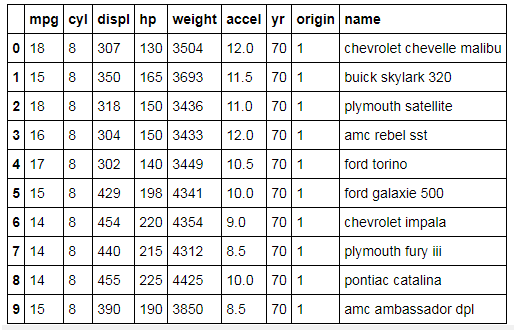
\includegraphics[width=\linewidth,keepaspectratio]{bk1}
\end{center}

\end{frame}

%%%%%%%%%%%%%%%%%%%%%%%%%%%%%%%%%%%%%%%%%%%%%%%%%%%
\begin{frame}[fragile] \frametitle{Bar Plot Example}
\begin{itemize}
\item For each year, we want to plot the distribution of MPG within that year. 
\item As a guide, we will include a box that represents the mean efficiency, plus and minus one standard deviation. 
\item We will make these boxes partly transparent.
\end{itemize}
\begin{lstlisting}
bk.hold(True)
bk.figure(title='Automobile mileage by year and country')
bk.quad(left=years-0.4, right=years+0.4, bottom=mpg_avg-mpg_std, top=mpg_avg+mpg_std, fill_alpha=0.4)
\end{lstlisting}
\end{frame}

%%%%%%%%%%%%%%%%%%%%%%%%%%%%%%%%%%%%%%%%%%%%%%%%%%%
\begin{frame}[fragile] \frametitle{Bar Plot Example}
We overplot the actual data points, using contrasting symbols for American and Japanese cars.
\begin{lstlisting}
# Add Japanese cars as circles
bk.circle(x=np.asarray(japanese["yr"]), 
       y=np.asarray(japanese["mpg"]), 
       size=8, alpha=0.4, line_color="red", fill_color=None, line_width=2)

# Add American cars as triangles
bk.triangle(x=np.asarray(american["yr"]), 
         y=np.asarray(american["mpg"]),
         size=8, alpha=0.4, line_color="blue", fill_color=None, line_width=2)
\end{lstlisting}
\end{frame}

%%%%%%%%%%%%%%%%%%%%%%%%%%%%%%%%%%%%%%%%%%%%%%%%%%%
\begin{frame}[fragile] \frametitle{Bar Plot Example}
We can add axis labels by binding them to the axis\_label attribute of each axis.
\begin{lstlisting}
xax, yax = bk.axis()
xax.axis_label = 'Year'
yax.axis_label = 'MPG'

bk.hold(False)
bk.show()
\end{lstlisting}
\end{frame}

%%%%%%%%%%%%%%%%%%%%%%%%%%%%%%%%%%%%%%%%%%%%%%%%%%%
\begin{frame}[fragile] \frametitle{Linked Brushing}
To link plots together at a data level, we can explicitly wrap the data in a ColumnDataSource. This allows us to reference columns by name.
\begin{lstlisting}
source = bk.ColumnDataSource(autompg.to_dict("list"))
source.add(autompg["yr"], name="yr")

plot_config = dict(plot_width=300, plot_height=300, tools="pan, wheel_zoom, box_zoom, select")
bk.gridplot([[
  bk.circle("yr", "mpg", color="blue", title="MPG by Year",
         source=source, **plot_config),
  bk.circle("hp", "displ", color="green", title="HP vs. Displacement",
         source=source, **plot_config),
  bk.circle("mpg", "displ", size="cyl", line_color="red", title="MPG vs. Displacement",
         fill_color=None, source=source, **plot_config)
  ]])
  bk.show()
\end{lstlisting}
\end{frame}


%%%%%%%%%%%%%%%%%%%%%%%%%%%%%%%%%%%%%%%%%%%%%%%%%%%
\begin{frame}[fragile] \frametitle{Visualization of US unemployment rates}
\begin{itemize}
\item Our first example of an interactive chart involves generating a heat map of US unemployment rates by month and year.
\item This plot will be made interactive by invoking a HoverTool that displays information as the pointer hovers over any cell within the plot.
\end{itemize}

\end{frame}


%%%%%%%%%%%%%%%%%%%%%%%%%%%%%%%%%%%%%%%%%%%%%%%%%%%
\begin{frame}[fragile] \frametitle{Visualization of US unemployment rates}
First, we import the data with Pandas and manipulate it as needed.
\begin{lstlisting}
import pandas as pd
from bokeh.objects import HoverTool
from bokeh.sampledata.unemployment1948 import data
from collections import OrderedDict

data['Year'] = [str(x) for x in data['Year']]
years = list(data['Year'])
months = ["Jan","Feb","Mar","Apr","May","Jun","Jul","Aug","Sep","Oct","Nov","Dec"]
data = data.set_index('Year')
\end{lstlisting}

\end{frame}

%%%%%%%%%%%%%%%%%%%%%%%%%%%%%%%%%%%%%%%%%%%%%%%%%%%
\begin{frame}[fragile] \frametitle{Visualization of US unemployment rates}
Specify a color map
\begin{lstlisting}
colors = [
    "#75968f", "#a5bab7", "#c9d9d3", "#e2e2e2", "#dfccce",
    "#ddb7b1", "#cc7878", "#933b41", "#550b1d"
]

month = []
year = []
color = []
rate = []
for y in years:
    for m in months:
        month.append(m)
        year.append(y)
        monthly_rate = data[m][y]
        rate.append(monthly_rate)
        color.append(colors[min(int(monthly_rate)-2, 8)])
\end{lstlisting}

\end{frame}

%%%%%%%%%%%%%%%%%%%%%%%%%%%%%%%%%%%%%%%%%%%%%%%%%%%
\begin{frame}[fragile] \frametitle{Visualization of US unemployment rates}
Create a ColumnDataSource with columns: month, year, color, rate
\begin{lstlisting}
source = bk.ColumnDataSource(
    data=dict(
        month=month,
        year=year,
        color=color,
        rate=rate,
    )
)

\end{lstlisting}

\end{frame}

%%%%%%%%%%%%%%%%%%%%%%%%%%%%%%%%%%%%%%%%%%%%%%%%%%%
\begin{frame}[fragile] \frametitle{Visualization of US unemployment rates}
\begin{itemize}
\item x\_range is years, y\_range is months (reversed)
\item fill color for the rectangles is the 'color' field
\item line\_color for the rectangles is None
\item tools are resize and hover tools
\item add a nice title, and set the plot\_width and plot\_height
\end{itemize}
\begin{lstlisting}
bk.rect('year', 'month', 0.95, 0.95, source=source,
     x_axis_location="above",
     x_range=years, y_range=list(reversed(months)),
     color='color', line_color=None,
     tools="resize,hover", title="US Unemployment (1948 - 2013)",
     plot_width=900, plot_height=400)
\end{lstlisting}
\end{frame}

%%%%%%%%%%%%%%%%%%%%%%%%%%%%%%%%%%%%%%%%%%%%%%%%%%%
\begin{frame}[fragile] \frametitle{Visualization of US unemployment rates}
Style the plot, including:
\begin{itemize}
\item remove the axis and grid lines
\item remove the major ticks
\item make the tick labels smaller
\item set the x-axis orientation to vertical, or angled
\end{itemize}
\begin{lstlisting}
bk.grid().grid_line_color = None
bk.axis().axis_line_color = None
bk.axis().major_tick_line_color = None
bk.axis().major_label_text_font_size = "5pt"
bk.axis().major_label_standoff = 0
bk.xaxis().major_label_orientation = np.pi/3
\end{lstlisting}
\end{frame}

%%%%%%%%%%%%%%%%%%%%%%%%%%%%%%%%%%%%%%%%%%%%%%%%%%%
\begin{frame}[fragile] \frametitle{Visualization of US unemployment rates}
Configure the hover tool to display the month, year and rate
\begin{itemize}
\item remove the axis and grid lines
\item remove the major ticks
\item make the tick labels smaller
\item set the x-axis orientation to vertical, or angled
\end{itemize}
\begin{lstlisting}
hover = bk.curplot().tools[1]
hover.tooltips = OrderedDict([
    ('date', '@month @year'),
    ('rate', '@rate'),
])
bk.show()
\end{lstlisting}
\end{frame}

%%%%%%%%%%%%%%%%%%%%%%%%%%%%%%%%%%%%%%%%%%%%%%%%%%%
\begin{frame}[fragile] \frametitle{High-level Plots}
\begin{itemize}
\item The examples so far have been relatively low-level, in that individual elements of plots need to be specified by hand. 
\item The bokeh.charts interface makes it easy to get up-and-running with a high-level API that tries to make smart layout and design decisions by default.
\end{itemize}
\end{frame}

%%%%%%%%%%%%%%%%%%%%%%%%%%%%%%%%%%%%%%%%%%%%%%%%%%%
\begin{frame}[fragile] \frametitle{High-level Plots}
To use them, you simply import the chart type you need from bokeh.charts:
\begin{itemize}
\item Bar
\item BoxPlot
\item HeatMap
\item Histogram
\item Scatter
\item Timeseries
\end{itemize}
\end{frame}

%%%%%%%%%%%%%%%%%%%%%%%%%%%%%%%%%%%%%%%%%%%%%%%%%%%
\begin{frame}[fragile] \frametitle{High-level Plots}
To illustrate, let's create some random data and display it as histograms.
\begin{lstlisting}
normal = np.random.standard_normal(1000)
student_t = np.random.standard_t(6, 1000)
distributions = pd.DataFrame({'Normal': normal, 'Student-T': student_t})

from bokeh.charts import Histogram

hist = Histogram(distributions, bins=np.sqrt(len(normal)), notebook=True)
hist.title("Histograms").ylabel("frequency").legend(True).width(600).height(300)

hist.show()
\end{lstlisting}
\end{frame}

%%%%%%%%%%%%%%%%%%%%%%%%%%%%%%%%%%%%%%%%%%%%%%%%%%%
\begin{frame}[fragile] \frametitle{Scatter Plot}
\begin{lstlisting}
from collections import OrderedDict

from bokeh.charts import Scatter
from bokeh.sampledata.iris import flowers

setosa = flowers[(flowers.species == "setosa")][["petal_length", "petal_width"]]
versicolor = flowers[(flowers.species == "versicolor")][["petal_length", "petal_width"]]
virginica = flowers[(flowers.species == "virginica")][["petal_length", "petal_width"]]

xyvalues = OrderedDict([("setosa", setosa.values), 
                        ("versicolor", versicolor.values), 
                        ("virginica", virginica.values)])

scatter = Scatter(xyvalues)
scatter.title("iris dataset, dict_input").xlabel("petal_length").ylabel("petal_width").legend("top_left")
scatter.width(600).height(400).notebook().show()
\end{lstlisting}
\end{frame}

%%%%%%%%%%%%%%%%%%%%%%%%%%%%%%%%%%%%%%%%%%%%%%%%%%%
\begin{frame}[fragile] \frametitle{Interactivity with other packages}
\begin{itemize}
\item Bokeh plots are compatible with other Python plotting packages, such as Matplotlib, Seaborn, and ggplot, via an onboard compatibility layer bokeh.mpl. 
\item This allows existing plots in these packages to be converted seamlessly into Bokeh.
\end{itemize}
\begin{lstlisting}
titanic = pd.read_csv('http://biostat.mc.vanderbilt.edu/wiki/pub/Main/DataSets/titanic3.csv')

\end{lstlisting}
\end{frame}

%%%%%%%%%%%%%%%%%%%%%%%%%%%%%%%%%%%%%%%%%%%%%%%%%%%
\begin{frame}[fragile] \frametitle{Interactivity with other packages}
\begin{lstlisting}
from ggplot import ggplot, aes, geom_density
from bokeh import mpl
import matplotlib.pyplot as plt

g = ggplot(titanic, aes(x='age', color='pclass')) + geom_density()

g.draw()

plt.title("Plot of titanic passenger age distribution by class")

mpl.to_bokeh(name="density")
\end{lstlisting}
\end{frame}

%%%%%%%%%%%%%%%%%%%%%%%%%%%%%%%%%%%%%%%%%%%%%%%%%%%
\begin{frame}[fragile] \frametitle{Interactivity with other packages}
\begin{lstlisting}
import seaborn as sns

# We generated random data
titanic = titanic.dropna(subset=['age'])

# And then just call the violinplot from Seaborn
sns.violinplot(titanic.age, groupby=titanic.pclass, color="Set3")

plt.title("Distribution of age by passenger class")

mpl.to_bokeh(name="violin")
\end{lstlisting}
\end{frame}

%%%%%%%%%%%%%%%%%%%%%%%%%%%%%%%%%%%%%%%%%%%%%%%%%%%
\begin{frame}[fragile] \frametitle{Generating and displaying images}
\begin{itemize}
\item Mandelbrot set images are made by sampling complex numbers and determining for each whether the result tends towards infinity when a particular mathematical operation is iterated on it.
\item First, functions for generating the Mandelbrot set image. They create a 2D array of numbers, over which a color map can be displayed.
\end{itemize}
\end{frame}

%%%%%%%%%%%%%%%%%%%%%%%%%%%%%%%%%%%%%%%%%%%%%%%%%%%
\begin{frame}[fragile] \frametitle{Generating and displaying images}
\begin{lstlisting}
def mandel(x, y, max_iters):
    """
    Given the real and imaginary parts of a complex number,
    determine if it is a candidate for membership in the Mandelbrot
    set given a fixed number of iterations.
    """
    c = complex(x, y)
    z = 0.0j
    for i in range(max_iters):
        z = z*z + c
        if (z.real*z.real + z.imag*z.imag) >= 4:
            return i
    return max_iters
\end{lstlisting}
\end{frame}

%%%%%%%%%%%%%%%%%%%%%%%%%%%%%%%%%%%%%%%%%%%%%%%%%%%
\begin{frame}[fragile] \frametitle{Generating and displaying images}
\begin{lstlisting}
def create_fractal(min_x, max_x, min_y, max_y, image, iters):
    height = image.shape[0]
    width = image.shape[1]

    pixel_size_x = (max_x - min_x) / width
    pixel_size_y = (max_y - min_y) / height

    for x in range(width):
        real = min_x + x * pixel_size_x
        for y in range(height):
            imag = min_y + y * pixel_size_y
            color = mandel(real, imag, iters)
            image[y, x] = color
\end{lstlisting}
\end{frame}

%%%%%%%%%%%%%%%%%%%%%%%%%%%%%%%%%%%%%%%%%%%%%%%%%%%
\begin{frame}[fragile] \frametitle{Generating and displaying images}
Define the bounding coordinates to generate the Mandelbrot image, then create a scalar image (2D array of numbers)
\begin{lstlisting}
min_x = -2.0
max_x = 1.0
min_y = -1.0
max_y = 1.0

img = np.zeros((1024, 1536), dtype = np.uint8)
create_fractal(min_x, max_x, min_y, max_y, img, 20)
\end{lstlisting}
\end{frame}

%%%%%%%%%%%%%%%%%%%%%%%%%%%%%%%%%%%%%%%%%%%%%%%%%%%
\begin{frame}[fragile] \frametitle{Generating and displaying images}
Use image renderer to display Mandelbrot image, colormapped with "Spectral-11" color palette. The renderer can display many images at once, so it takes lists of images, coordinates, and palettes.
\begin{lstlisting}
bk.image(image=[img],
      x=[min_x],
      y=[min_y],
      dw=[max_x-min_x],
      dh=[max_y-min_y],
      palette=["Spectral-11"],
      x_range = [min_x, max_x],
      y_range = [min_y, max_y],
      title="Mandelbrot",
      tools="pan,wheel_zoom,box_zoom,reset,previewsave",
      plot_width=900,
      plot_height=600
)
bk.show()
\end{lstlisting}
\end{frame}









